% Revised manuscript, v8.
% Target venue: EUMAS 2026 / Springer LNCS.
\documentclass[runningheads]{llncs}

\usepackage[T1]{fontenc}
\usepackage{graphicx}
\usepackage{amsmath,amssymb}
\usepackage{booktabs}
\usepackage{array}
\usepackage{url}
\usepackage{xcolor}
\setlength{\textfloatsep}{7pt plus 1pt minus 2pt}
\setlength{\floatsep}{7pt plus 1pt minus 2pt}
\setlength{\intextsep}{7pt plus 1pt minus 2pt}
\setlength{\abovecaptionskip}{3pt}
\setlength{\belowcaptionskip}{0pt}
\emergencystretch=2em

\newcommand{\ind}{\mathbb{I}}
\newcommand{\clip}{\operatorname{clip}}
\newcommand{\argmaxop}{\operatorname*{arg\,max}}

\begin{document}

\title{Emotionally Bounded-Rational Agents in Repeated Games:\
An Interpretable Dual-System Architecture and Diagnostic Calibration Study}
\titlerunning{Emotionally Bounded-Rational Agents in Repeated Games}

\author{Dmitri Pavliuchenkov\inst{1}\thanks{Corresponding author.} \and Dmitri Gubanov\inst{2}}
\authorrunning{D. Pavliuchenkov and D. Gubanov}
\institute{Moscow Institute of Physics and Technology, Dolgoprudny, Russia\\
\email{pavliuchenkov.dm@phystech.edu}
\and
Institute for Control Sciences RAS, Moscow, Russia}

\maketitle

\begin{abstract}
Repeated social interaction is rarely reducible to payoff maximization alone: the same material outcome can be evaluated differently depending on fairness, relationship history, perceived vulnerability, affective activation, and fatigue. We conceptualize emotionally bounded-rational agents as agents whose decisions are shaped by subjective value appraisal, fatigue-dependent emotional dominance, and the cost of regulating emotional impulses. We present an interpretable, implementation-aware dual-system architecture for repeated games. A game-to-values adapter maps game-specific outcomes into a shared internal value space: material payoff, fairness, relationship quality, and safety. A fast affective System~1 proposes action tendencies, while a slower System~2 can accept, override, or refocus them in order to preserve an overall internal-state score. The paper is framed as an architectural and diagnostic calibration study rather than as a claim of final behavioral validation. Using the corrected experiment runner and new paper-profile runs, we report 20-episode, 200-round experiments across the Prisoner's Dilemma, Battle of the Sexes, and Ultimatum Game. The results replace isolated examples with reproducible cross-type matchups, fixed-strategy adaptation proxies, affective-profile sweeps, and internal-state diagnostics. They show no universal dominance of hybrid agents, but they do show that payoff, social game metrics, and internal state can diverge sharply. The contribution is a self-contained computational specification and artifact-backed diagnostic pipeline with explicit implementation-status boundaries for studying when emotionally bounded-rational mechanisms are informative, fragile, or still under-specified.
\keywords{Bounded rationality \and Emotional regulation \and Multi-agent simulation \and Repeated games \and Game-to-values adapter \and Diagnostic experiments}
\end{abstract}

\section{Introduction}

Classical agent-based models and reinforcement-learning systems often represent strategic choice as the maximization of a single payoff or reward. This abstraction is useful for formal analysis, but it is too narrow for simulating social interaction. In repeated settings, agents evaluate not only what they obtained, but also whether the interaction was fair, whether the partner supported or exploited them, whether cooperation made them vulnerable, and how costly it is to regulate emotional responses over time.

This paper addresses the problem of over-rationalized agents in repeated games. We do not merely add an ``emotion variable'' to a payoff optimizer. Instead, we separate the external game outcome from its subjective interpretation by the agent. A joint action first produces payoff and an outcome in the external environment. The outcome is then interpreted as a vector of internal event values: material payoff, fairness, relationship quality, and safety. Changes in these values drive appraisal, mood, fatigue, and well-being, which in turn affect the next action.

The architecture is inspired by bounded rationality~\cite{simon1955behavioral}, dual-process decision-making~\cite{kahneman2011thinking}, prospect theory~\cite{kahneman1979prospect}, affective computing~\cite{picard1997affective}, appraisal theories of emotion~\cite{ortony1988cognitive,marsella2009ema}, and reinforcement learning~\cite{sutton2018reinforcement,mnih2015human}. Repeated games are used as a compact diagnostic testbed because they make payoff, fairness, coordination, exploitation, and adaptation observable under controlled conditions.

We make three methodological commitments. First, the terms \emph{optimistic}, \emph{neutral}, and \emph{pessimistic} denote parameterized affective profiles, not validated psychological personality types. Second, the reported runs are diagnostic rather than confirmatory: they inspect mechanisms and failure modes, not statistical superiority. Third, the architecture does not eliminate scalarization. It relocates scalarization from raw payoff to a transparent internal-state score after value interpretation and affective-state updating.

We organize the paper around four research questions:
\begin{itemize}
    \item \textbf{RQ1:} Can one value-based affective-rational specification be applied across several repeated games?
    \item \textbf{RQ2:} How do hybrid, rational, emotional, and fixed-strategy agents differ in payoff, game-specific metrics, and internal-state stability?
    \item \textbf{RQ3:} Is there descriptive evidence of adaptation to fixed partners between the first and last third of an episode?
    \item \textbf{RQ4:} Which current mechanisms appear to contribute to internal-state collapse?
\end{itemize}

The contributions are: (i) a formal but implementation-aware specification of emotionally bounded-rational agents; (ii) a game-to-values adapter that links external outcomes to internal value dimensions; (iii) a dual-system decision loop with emotional dominance, rational override, fatigue, and refocus; and (iv) a paper-profile diagnostic experiment package with game-specific metrics, state trajectories, and explicit limits on interpretation.

\section{Related Work}

The work is positioned at the intersection of three research directions. The first is bounded rationality and social decision-making in games. Simon's account of bounded rationality~\cite{simon1955behavioral}, Kahneman's fast/slow distinction~\cite{kahneman2011thinking}, and prospect theory~\cite{kahneman1979prospect} motivate models in which salience, loss, affect, and context shape decisions instead of a single ideal utility calculation. Game-theoretic baselines remain essential: Nash equilibrium~\cite{nash1950equilibrium}, Axelrod's analysis of cooperation and tit-for-tat~\cite{axelrod1984evolution}, and behavioral models of fairness, inequity aversion, guilt, and punishment~\cite{guth1982ultimatum,fehr1999theory,rabin1993fairness,battigalli2007guilt,battigalli2022belief,fehr2002punishment} frame our use of repeated games and internal value dimensions.

The second direction is affective agent architecture. Existing systems include OCC-style appraisal~\cite{ortony1988cognitive}, EMA~\cite{marsella2009ema}, ALMA~\cite{gebhard2005alma}, WASABI~\cite{beckerasano2010wasabi}, FAtiMA~\cite{dias2014fatima}, and MAMID~\cite{hudlicka2004mamid}; emotion in reinforcement learning has also been surveyed in robotics and RL~\cite{moerland2018emotion}. Our contribution is narrower than a complete cognitive architecture: we build a compact repeated-game prototype in which value interpretation, mood, fatigue, well-being, and appraisal diagnostics are explicit and inspectable.

The third direction is multi-agent learning in social dilemmas. Modern MARL emphasizes non-stationarity, cooperation, communication, contracts, and evaluation~\cite{gronauer2022marl,zhu2024communication,ning2024survey,mu2024socialdilemmas,willis2024reward,haupt2024contracts,su2026iterated}. These works motivate caution: claims about repeated-game adaptation require longer horizons, multiple seeds, and game-sensitive metrics. We therefore present the experiments as diagnostic calibration rather than as convergence or state-of-the-art performance evidence.

\section{Model Specification}

The model is a closed affective-cognitive loop. An agent observes a repeated-game state, selects an action, receives an external outcome and material payoff, interprets that outcome through value dimensions, updates internal state variables, and uses the updated state in subsequent decisions. This section first defines the external game and the game-to-values adapter, then the internal state variables, and finally the appraisal quantities used to interpret changes in values. Section~4 then explains how these quantities enter the two-system control loop. Figure~\ref{fig:architecture} gives the same story visually and separates the conceptual pipeline from the mechanisms that are behavior-driving in the current paper runs.

\subsection{External Game and Value Interpretation}

A repeated game is modeled as an external environment
\[
G=(N,\mathcal{S},\mathcal{A},T,R,\Omega),
\]
where $N$ is the set of agents, $\mathcal{S}$ the game-state space, $\mathcal{A}=(\mathcal{A}_i)_{i\in N}$ the family of legal action sets, $T$ the transition/outcome rule, $R=(R_i)_{i\in N}$ the family of material payoff functions, and $\Omega$ the outcome space. At step $t$, agent $i$ chooses $a_{i,t}\in\mathcal{A}_i$, the environment returns outcome $o_t\in\Omega$, and the material payoff is $\pi_{i,t}=R_i(o_t)$.

The game-to-values adapter separates the external result from its subjective meaning for the agent:
\[
A_i^G(a_i,a_j,\pi_i,\pi_j)\rightarrow q_i=(q_i^{mat},q_i^{fair},q_i^{rel},q_i^{safe})\in[0,1]^4.
\]
Table~\ref{tab:values} defines these event values. In the conceptual model, event values are the bridge from external outcomes to accumulated internal values. In the current paper-profile implementation, the learned agents already have behavior-relevant internal state variables such as mood, fatigue, well-being, and overall state; the additional adapter/appraisal quantities are computed from logged outcomes as diagnostic variables. Thus they help explain the runs reported here, but they do not feed back into action selection in these paper-profile experiments.

\begin{table}[t]
\centering
\caption{Subjective event values returned by the game-to-values adapter.}
\label{tab:values}
\scriptsize
\begin{tabular}{p{0.18\linewidth}p{0.27\linewidth}p{0.29\linewidth}p{0.16\linewidth}}
\toprule
Value & Meaning & Operational proxy & Role \\
\midrule
Material payoff & Agent's material outcome. & Payoff normalized by the feasible payoff range of the agent in the game. & Links the model to classical game payoffs. \\
Fairness & Perceived symmetry of the outcome. & $1-|\tilde{\pi}_i-\tilde{\pi}_j|$, using normalized payoffs. & Captures unfairness and bargaining sensitivity. \\
Relationship & Whether the partner supported or harmed the agent given the agent's action. & Actual payoff relative to best/worst payoff obtainable under the observed partner action. & Represents trust, betrayal, and repair. \\
Safety & Protection from exploitation or regret. & $1-$ normalized regret relative to the best response to the partner's action. & Captures vulnerability in repeated interaction. \\
\bottomrule
\end{tabular}
\end{table}

\subsection{Internal State and Implementation Status}

Each agent maintains an internal value state $v_i(t)\in[0,1]^4$, priorities $p_i$ with $\sum_k p_{i,k}=1$, mood $m_i(t)$, fatigue $f_i(t)$, well-being $w_i(t)$, and overall state score $S_i(t)$. Well-being is the weighted degree of value satisfaction:
\[
w_i(t)=\sum_k p_{i,k}v_{i,k}(t).
\]
The overall state score is an interpretable first-order aggregation:
\[
S_i(t)=\lambda_w w_i(t)+\lambda_m m_i(t)-\lambda_f f_i(t).
\]
This is not a psychometric claim about subjective well-being. It is a computational score used to audit how payoff-seeking, mood, fatigue, and value satisfaction interact.

\begin{table}[t]
\centering
\caption{Status of major mechanisms in the current article.}
\label{tab:implstatus}
\scriptsize
\begin{tabular}{p{0.30\linewidth}p{0.23\linewidth}p{0.37\linewidth}}
\toprule
Component & Status in paper runs & Role in this article \\
\midrule
Learned two-system agents & Behavior-driving & Core policy mechanism for hybrid, emotional, and rational comparisons. \\
Mood, fatigue, well-being, overall state & Behavior-driving/logged & Part of the agent state and the main source of internal-state diagnostics. \\
Game-to-values adapter & Diagnostic/explanatory layer & Computes event-value interpretations from logged outcomes; it is used to explain results, not to change actions in these paper-profile runs. \\
Appraisal variables: urgency, valence, load, focus & Diagnostic/explanatory layer & Derived from value changes to analyze why state collapse or payoff-state divergence occurs. \\
Suppression-cost proxy & Diagnostic proxy & Used to interpret regulation costs; not a fully behavior-driving fatigue mechanism in the reported runs. \\
\bottomrule
\end{tabular}

\end{table}

Table~\ref{tab:implstatus} is intentionally conservative. Behavior-driving variables affect the reported runs. Diagnostic variables are derived from logs to explain and audit outcomes; they are not mood, fatigue, or well-being themselves, and they do not change the policies in the paper-profile experiments. Future mechanisms such as belief update and a fully white-box bounded-rational agent are mentioned only in the conclusion and threats to validity.

\subsection{Urgency, Valence, Emotional Load, and Focus}

For each value $k$, urgency measures the subjective criticality of a value change. If $\Delta v_{i,k}(t)=v_{i,k}(t)-v_{i,k}(t-1)$, then one practical bounded form is
\[
u_{i,k}(t)=
\begin{cases}
\min\left(1,\dfrac{|\Delta v_{i,k}(t)|}{\max(\epsilon,1-v_{i,k}(t-1))}\right), & \Delta v_{i,k}(t)>0,\\[7pt]
\min\left(1,\dfrac{|\Delta v_{i,k}(t)|}{\max(\epsilon,v_{i,k}(t-1))}\right), & \Delta v_{i,k}(t)<0,\\[7pt]
0, & \Delta v_{i,k}(t)=0.
\end{cases}
\]
Signed urgency is $\operatorname{sgn}(\Delta v_{i,k})u_{i,k}$. Valence and emotional load are
\[
V_i(t)=\sum_k p_{i,k}\operatorname{sgn}(\Delta v_{i,k})u_{i,k},\qquad
L_i(t)=\sum_k p_{i,k}u_{i,k}.
\]
Valence captures the direction of appraisal, while emotional load captures intensity regardless of sign. Attention focus is $k^*_i(t)=\argmaxop_k p_{i,k}u_{i,k}$.

\section{Dual-System Control and Implementation Status}

The paper uses the term \emph{DQN-like} for the learned action-selection modules. Operationally, each module receives a numeric state vector, selects an action or control option using an epsilon-greedy policy over learned $Q$-values, stores transitions in a replay buffer, and updates a neural network by minibatch Bellman-style targets with a slower target network. In the hybrid agent, System~1 and System~2 are separate trainable modules; in the rational baseline, emotional influence is neutralized for action selection. Because each reported episode has 200 rounds, these modules are treated as trainable prototype policies, not as fully converged deep-RL solutions.

\subsection{Decision Rule, Regulation, and Fatigue}

System~1 is the fast affective mechanism. In the learned implementation it proposes an emotional action tendency with valenced intensity. In the formal specification, System~1 reacts to attention focus and valence. System~2 is the slower control mechanism. It accepts, overrides, or refocuses the emotional proposal and is trained to improve the overall internal-state score.

An emotional impulse dominates if its intensity exceeds a fatigue-dependent threshold:
\[
\theta_i(t)=\clip\left(\theta_{0,i}(1-\lambda_f f_i(t)),\theta_{min},\theta_{max}\right).
\]
Thus fatigue reduces the ability to suppress emotional impulses. If System~2 suppresses an emotional proposal, regulation is costly:
\[
C^{sup}_i(t)=\gamma\,\ind[a^{final}_{i,t}\neq a^{EM}_{i,t}]\,|e_{i,t}|.
\]
A compact fatigue update is
\[
f_i(t+1)=(1-\rho)f_i(t)+\rho\left(\beta L_i(t)+(1-\beta)C^{sup}_i(t)\right).
\]
A fully white-box bounded-rational agent that follows these equations directly remains a future validation baseline, not a current result.


\begin{table}[t]
\centering
\caption{Compact one-step decision/update pipeline used to align the formal model with the implementation.}
\label{tab:pipeline}
\scriptsize
\begin{tabular}{p{0.08\linewidth}p{0.84\linewidth}}
\toprule
Step & Operation \\
\midrule
1 & Observe game state, legal actions, previous value changes, mood, fatigue, and current internal state. \\
2 & System~1 proposes an affective action tendency and an emotion intensity from appraisal-related inputs. \\
3 & Compare impulse intensity with the fatigue-dependent threshold; if it dominates, execute the emotional action. \\
4 & Otherwise System~2 accepts, overrides, or refocuses the proposal according to the overall-state objective. \\
5 & Execute joint actions in the external game and observe payoffs/outcome. \\
6 & Apply the game-to-values adapter, update internal values and state variables, log diagnostics, and store training transitions. \\
\bottomrule
\end{tabular}
\end{table}

Table~\ref{tab:pipeline} also clarifies the time ordering: current action selection uses previous state and previous appraisals; newly observed outcomes update values and diagnostics for the next step.

\begin{figure}[t]
\centering
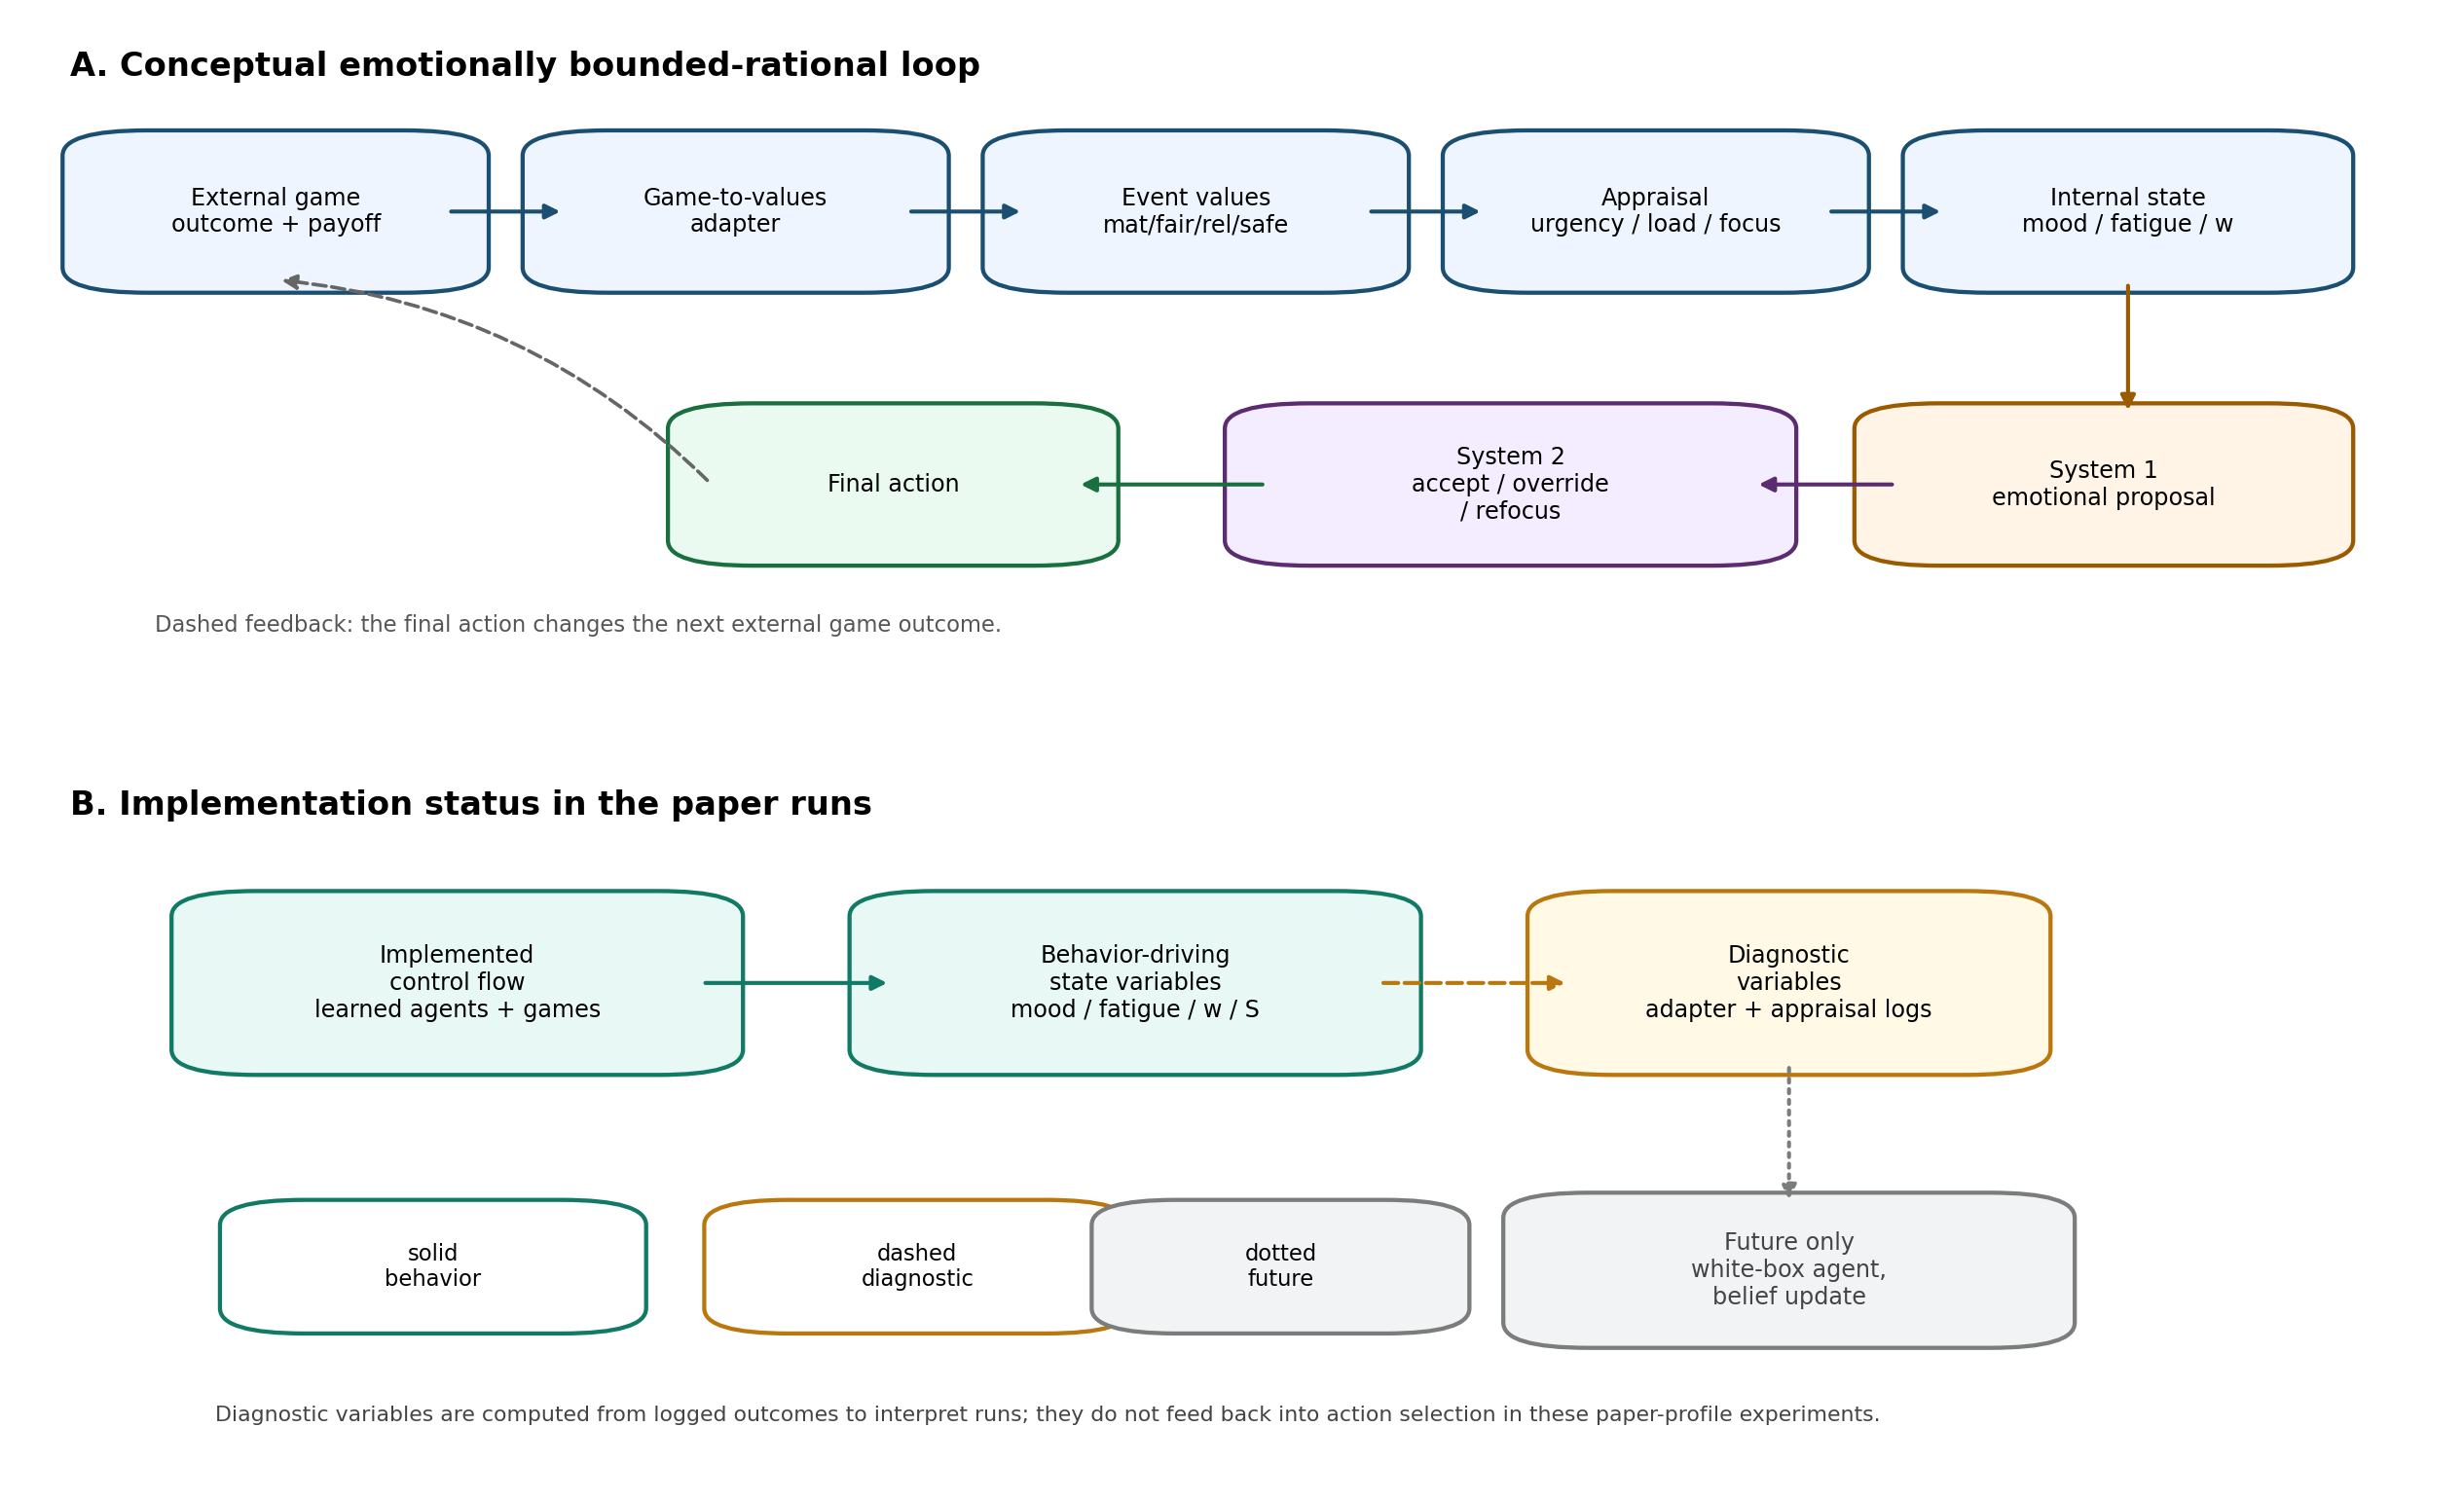
\includegraphics[width=0.92\linewidth]{figures/architecture_concept_status_v8.png}
\caption{Conceptual and implementation-aware architecture. Panel A shows the emotionally bounded-rational pipeline: external outcomes are mapped into subjective values, appraisal, internal state, System~1/System~2 control, and final action. Panel B separates behavior-driving control flow from diagnostic interpretation and future-only elements. Solid arrows denote behavior-driving mechanisms in the paper runs, dashed arrows denote diagnostic interpretation, and dotted/grey elements denote future-only mechanisms.}
\label{fig:architecture}
\end{figure}

\section{Experimental Protocol}

The new paper-profile experiments use the latest corrected runner and code snapshot. The artifact bundle contains S1--S4 paper runs plus smoke and standard validation runs. One episode is a complete repeated interaction under a fixed game, agent pair, configuration, and seed; one round is a single stage-game interaction inside that episode. All main paper runs use 20 independent episodes and 200 rounds per condition. Ordered pairs are kept distinct because role, payoff split, and agent-specific internal state can differ between, for example, Hybrid--Rational and Rational--Hybrid. Table~\ref{tab:protocol} summarizes the main runs and the validation report states that the bundle passed the expected file, table, plot, and log checks.

\begin{table}[t]
\centering
\caption{Main paper-profile experimental scenarios. ``All'' denotes PD, BoS, and UG; conditions are distinct agent-pair/game settings and plots are automatically generated article diagnostics.}
\label{tab:protocol}
\scriptsize
\begin{tabular}{llccccc}
\toprule
Scenario & Purpose & Games & Episodes & Rounds & Conditions & Plots \\
\midrule
S1 & Ordered cross-type matrix & all & 20 & 200 & 48 & 48 \\
S2 & Fixed-strategy adaptation proxy & all & 20 & 200 & 27 & 152 \\
S3 & Profile $\times$ intensity sweep & PD & 20 & 200 & 27 & 18 \\
S3 optional & Profile sweep robustness & all & 20 & 200 & 81 & 48 \\
S4 & Internal-state dynamics & all & 20 & 200 & 12 & 168 \\
\bottomrule
\end{tabular}

\end{table}

The games are the Prisoner's Dilemma (PD), Battle of the Sexes (BoS), and Ultimatum Game (UG). Table~\ref{tab:method} summarizes their external action and payoff rules, paper-profile scale, and aggregation logic so that the experimental setup is readable without the supplementary archive. The outcome metrics are game-sensitive: mutual cooperation and exploitation in PD; agreement and turn-taking in BoS; offer level, fair-offer rate, and acceptance in UG. Internal-state metrics include mean and final overall state, negative-state share, mood/fatigue trajectories, and payoff--state correlations. Scenario S2 is treated cautiously: fixed-strategy action semantics are clearest in PD, while non-PD fixed-strategy matchups are stress tests and not central evidence.


\begin{table}[t]
\centering
\caption{Compact methodological details needed to read the experiments without the supplementary archive.}
\label{tab:method}
\scriptsize
\begin{tabular}{p{0.18\linewidth}p{0.30\linewidth}p{0.42\linewidth}}
\toprule
Block & Setting & Notes \\
\midrule
Paper runs & S1--S4; 20 episodes; 200 rounds & Episodes are independent repeated-game runs under one condition and seed; all values are descriptive means unless stated otherwise. \\
Games & PD, BoS, UG & PD uses $CC=(3,3)$, $CD=(0,5)$, $DC=(5,0)$, $DD=(1,1)$; BoS uses two asymmetric coordination outcomes; UG uses fixed proposer/responder roles, discretized offers, and accept/reject outcomes. \\
Conditions & Ordered agent pairs & Hybrid--Rational and Rational--Hybrid are distinct because split payoff and role-specific internal state matter. \\
Learning & DQN-like modules, replay, target network, $\gamma$-discounting, epsilon-greedy exploration & Used as trainable action-selection mechanisms; 200-round traces are not claimed as converged deep-RL policies. \\
State score & $S_i=w_i+m_i-f_i$ & Interpretable diagnostic aggregation, not a psychometric well-being scale. \\
Statistics & Means over 20 episodes; source CSVs in artifact bundle & No p-values; claims are diagnostic and calibration-oriented. \\
\bottomrule
\end{tabular}

\end{table}

Table~\ref{tab:method} summarizes external games, paper-profile scale, ordered conditions, learning settings, and aggregation. It also clarifies the ranges of the reported scenario counts: episodes and rounds are fixed by the paper profile, conditions count agent-pair/game configurations, and plots count generated diagnostic figures.

\section{Results}

Reading guide: S1 evaluates cross-type comparisons, S2 gives a first-vs-last-third adaptation proxy, S3 is an affective-profile calibration sweep, and S4 analyzes internal-state collapse. All claims are descriptive and calibration-oriented.

\subsection{S1: Cross-Type Matchups}

S1 contains 48 ordered conditions: three games times 16 ordered type-pairs. Table~\ref{tab:s1} reports representative conditions selected to show payoff, split payoff, and internal-state contrasts rather than only top scores. Mutual cooperation is the fraction of PD rounds in which both agents choose cooperation. Pair state is the mean of the two agents' mean overall-state scores $S_i$ within the condition. Figure~\ref{fig:s1tradeoff} visualizes the same payoff--state trade-off. The strongest lesson is not that the hybrid agent is universally better. Rather, the same condition can look favorable under payoff and unfavorable under internal-state stability.

\begin{table}[t]
\centering
\caption{Selected S1 comparisons from the paper-profile runs. Metric is mutual cooperation in PD, agreement in BoS, and acceptance rate in UG. Values are means over 20 episodes and 200 rounds.}
\label{tab:s1}
\scriptsize
\begin{tabular}{llcccc}
\toprule
Game & Pair & Pair payoff & Split & Pair state & Metric \\ 
\midrule
PD & Hybrid--Hybrid & 896.5 & 441.1/455.4 & -1.00 & 0.249 \\ 
PD & Hybrid--Rational & 832.8 & 313.5/519.2 & -0.62 & 0.157 \\ 
PD & Rational--Rational & 734.2 & 372.8/361.5 & -0.10 & 0.111 \\ 
PD & Emotional--Rational & 830.4 & 327.8/502.6 & -0.50 & 0.159 \\ 
PD & Fixed TFT--Fixed TFT & 1200.0 & 600.0/600.0 & -0.72 & 1.000 \\ 
\midrule
BoS & Hybrid--Hybrid & 492.0 & 245.2/246.8 & -1.08 & 0.492 \\ 
BoS & Hybrid--Rational & 477.2 & 226.1/251.2 & -0.73 & 0.477 \\ 
BoS & Rational--Rational & 550.8 & 265.2/285.6 & -0.40 & 0.551 \\ 
BoS & Emotional--Rational & 509.0 & 243.6/265.4 & -0.59 & 0.509 \\ 
BoS & Fixed TFT--Fixed TFT & 1000.0 & 600.0/400.0 & -0.82 & 0.000 \\ 
\midrule
UG & Hybrid--Hybrid & 697.5 & 341.8/355.8 & -1.03 & 0.349 \\ 
UG & Hybrid--Rational & 1183.0 & 572.1/610.9 & -0.62 & 0.592 \\ 
UG & Rational--Rational & 1162.5 & 591.5/571.0 & -0.17 & 0.581 \\ 
UG & Emotional--Rational & 1144.0 & 550.5/593.5 & -0.50 & 0.572 \\ 
UG & Fixed TFT--Fixed TFT & 0.0 & 0.0/0.0 & -0.72 & 0.000 \\ 
\bottomrule
\end{tabular}

\end{table}

\begin{figure}[t]
\centering
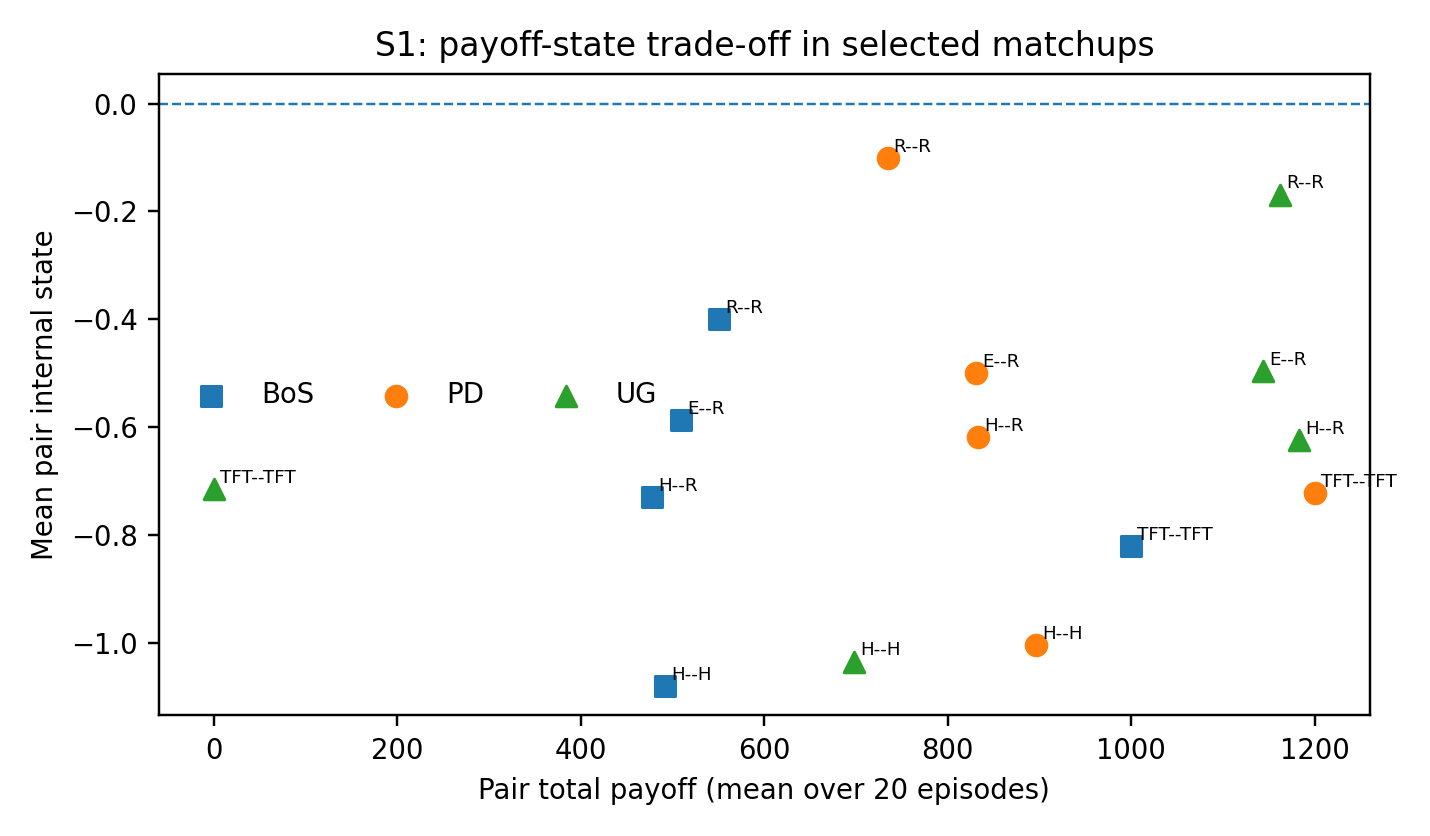
\includegraphics[width=0.78\linewidth]{figures/s1_payoff_state_tradeoff.png}
\caption{S1 payoff-state trade-off in selected conditions. High external payoff can coexist with strongly negative internal state, especially for affective agents.}
\label{fig:s1tradeoff}
\end{figure}

In PD, fixed tit-for-tat versus itself reaches the expected cooperative sanity-check outcome: pair payoff $1200$ and mutual cooperation $1.0$. Among learned agents, hybrid-hybrid obtains high pair payoff ($896.55$) but a strongly negative pair state. Hybrid versus rational is also high in pair payoff ($832.75$) but asymmetric: the rational agent receives $519.25$ while the hybrid agent receives $313.50$. This is better described as exploitation/asymmetry than as hybrid success.

In BoS, rational-rational outperforms hybrid-hybrid in payoff and internal state. In UG, hybrid-rational and rational-rational are the most informative selected conditions. Hybrid-rational has the highest selected pair payoff ($1183$), but the hybrid state remains strongly negative. These patterns support RQ2 only descriptively: game, partner, and metric determine which architecture looks preferable.

\subsection{S2: Adaptation to Fixed Strategies}

S2 compares the first and last third of each episode. Table~\ref{tab:s2pd} shows the PD subset, which is the safest adaptation proxy because fixed strategies map cleanly to cooperate/defect/tit-for-tat semantics.

\begin{table}[t]
\centering
\caption{S2 adaptation proxy in the Prisoner's Dilemma: last third minus first third. Cooperation is reported as first-to-last; $\Delta$ payoff is agent~1 payoff change.}
\label{tab:s2pd}
\scriptsize
\begin{tabular}{llccc}
\toprule
Agent & Fixed partner & Cooperation & $\Delta$ coop. & $\Delta$ payoff \\ 
\midrule
Emotional & Always-C & 0.488$\to$0.521 & 0.033 & -4.4 \\ 
Emotional & Always-D & 0.489$\to$0.530 & 0.041 & -2.7 \\ 
Emotional & TFT & 0.486$\to$0.530 & 0.043 & 1.8 \\ 
\midrule
Hybrid & Always-C & 0.505$\to$0.445 & -0.059 & 7.8 \\ 
Hybrid & Always-D & 0.499$\to$0.458 & -0.042 & 2.8 \\ 
Hybrid & TFT & 0.503$\to$0.471 & -0.032 & -7.8 \\ 
\midrule
Rational & Always-C & 0.452$\to$0.206 & -0.245 & 32.4 \\ 
Rational & Always-D & 0.427$\to$0.206 & -0.221 & 14.6 \\ 
Rational & TFT & 0.433$\to$0.211 & -0.223 & -36.4 \\ 
\bottomrule
\end{tabular}

\end{table}

Figure~\ref{fig:s2adapt} pairs the S2 payoff change with cooperation change in PD. The rational agent sharply reduces cooperation against fixed opponents and increases payoff against always-cooperate and always-defect, but loses payoff against tit-for-tat. The hybrid agent shows a milder cooperation decrease and modest payoff gains against always-cooperate and always-defect. The emotional agent increases cooperation and loses payoff against always-cooperate/always-defect. Thus RQ3 receives partial support only as a proxy: current agents adapt in measurable ways, but the direction is payoff-oriented for rational agents and mixed for affective agents. In UG, fixed-strategy conditions produce zero pair payoff and are treated as a technical limitation rather than substantive adaptation evidence.

\begin{figure}[t]
\centering
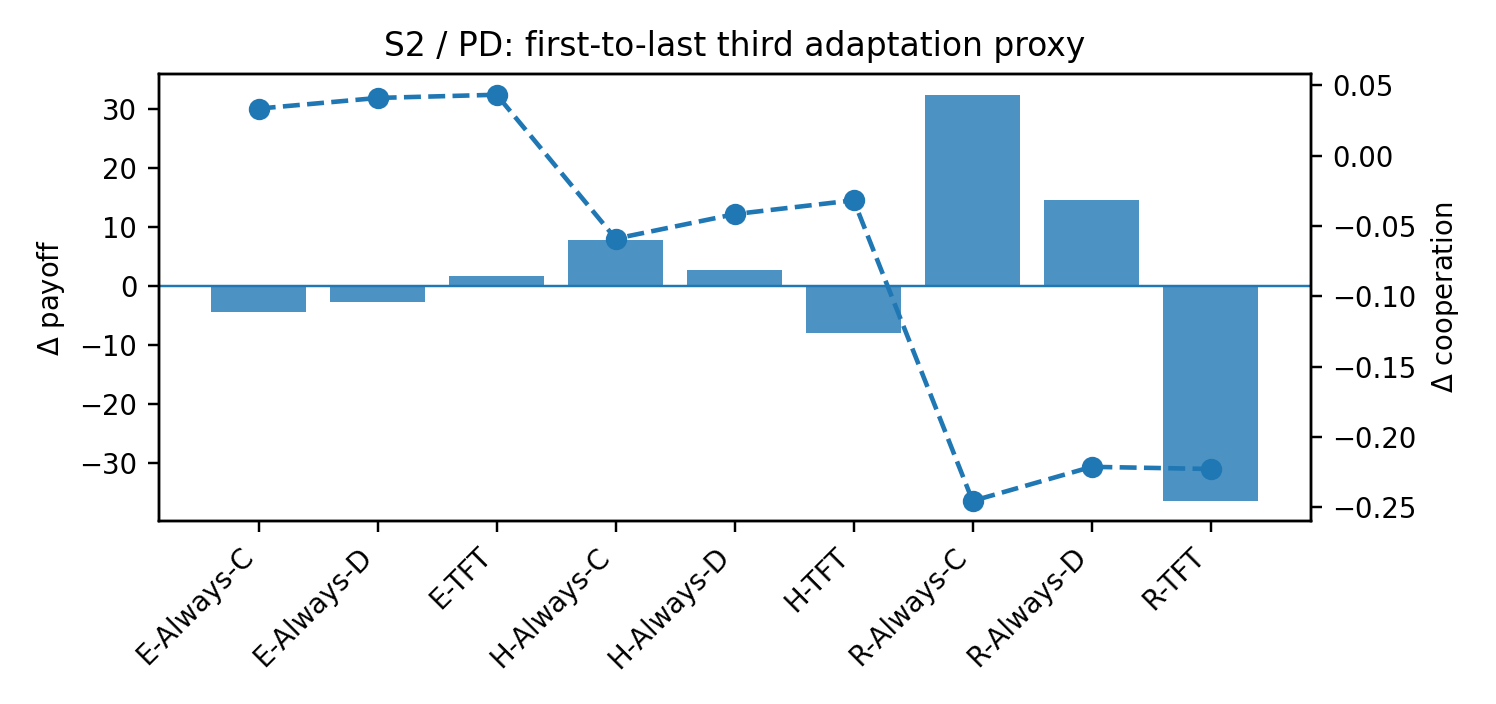
\includegraphics[width=0.72\linewidth]{figures/s2_pd_adaptation_proxy.png}
\caption{S2/PD adaptation proxy. Bars show payoff change; the dashed line shows cooperation change. Labels abbreviate agent type and fixed partner.}
\label{fig:s2adapt}
\end{figure}

\subsection{S3: Affective-Profile Calibration}

S3 is a calibration sweep over affective profile and emotional intensity, not a personality validation study. Figure~\ref{fig:s3profile} shows that profile differences are dominated by the broader negative-state regime; the full per-cell PD table is included in the artifact bundle. The largest pair payoff occurs for pessimistic-neutral and neutral-low cells, while the least negative internal states among high-payoff cells occur closer to optimistic-neutral or optimistic-high. The differences are moderate and should be interpreted as sensitivity analysis rather than stable psychological types.

\begin{figure}[t]
\centering
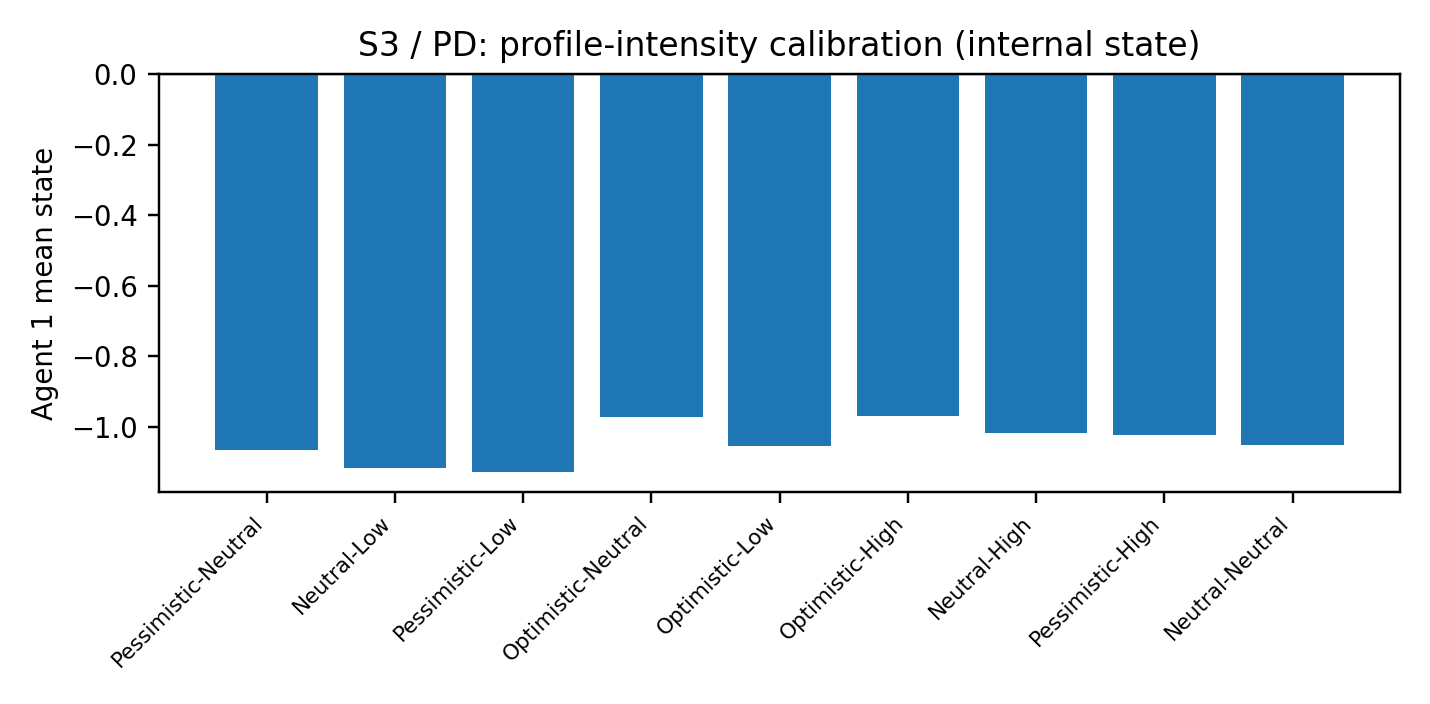
\includegraphics[width=0.70\linewidth]{figures/s3_pd_profile_state.png}
\caption{S3/PD profile-intensity calibration by internal state. All cells remain mostly negative; profile effects are weaker than the overall calibration problem.}
\label{fig:s3profile}
\end{figure}

Optional all-game S3 runs were also completed. They are useful for checking robustness, but UG fixed-opponent cells produce zero pair payoff and should not anchor substantive claims. This supports the experimental guardrail: S3 is informative for calibration and sensitivity, not for validating human-like personality dynamics.

\subsection{S4: Internal-State Diagnostics}

S4 is the most important diagnostic scenario. It contains 12 conditions over all games and shows that high or non-trivial payoff may coexist with degraded internal state. In Table~\ref{tab:s4}, A1 neg. is the share of rounds in which agent~1 has $S_1<0$. Its values are often close to one because the current internal-state calibration combines high targets, negative mood dynamics, and fatigue in a way that produces chronic negative regimes. This is a calibration diagnosis, not a claim that every action is externally unsuccessful. Table~\ref{tab:s4} summarizes the main conditions, while Figure~\ref{fig:s4collapse} shows the collapse pattern and negative-state share.

\begin{table}[t]
\centering
\caption{S4 internal-state diagnostics from the paper-profile runs. Metric is mutual cooperation in PD, agreement in BoS, and acceptance rate in UG.}
\label{tab:s4}
\scriptsize
\begin{tabular}{llccccc}
\toprule
Game & Pair & Payoff & A1 state & A2 state & A1 neg. & Metric \\ 
\midrule
PD & Hybrid--Rational & 832.8 & -1.008 & -0.227 & 0.998 & 0.157 \\ 
PD & Hybrid--Fixed D & 695.4 & -1.054 & -0.624 & 0.999 & 0.000 \\ 
PD & Hybrid--Fixed TFT & 884.1 & -1.062 & -0.640 & 0.999 & 0.258 \\ 
PD & Emotional--Rational & 830.4 & -0.809 & -0.190 & 0.999 & 0.159 \\ 
\midrule
BoS & Hybrid--Rational & 477.2 & -1.072 & -0.388 & 0.998 & 0.477 \\ 
BoS & Hybrid--Fixed D & 497.8 & -1.101 & -0.726 & 0.999 & 0.000 \\ 
BoS & Hybrid--Fixed TFT & 499.2 & -1.103 & -0.723 & 0.999 & 0.000 \\ 
BoS & Emotional--Rational & 509.0 & -0.798 & -0.375 & 0.999 & 0.509 \\ 
\midrule
UG & Hybrid--Rational & 1183.0 & -1.071 & -0.176 & 1.000 & 0.592 \\ 
UG & Hybrid--Fixed D & 0.0 & -0.999 & -0.752 & 0.999 & 0.000 \\ 
UG & Hybrid--Fixed TFT & 0.0 & -0.999 & -0.752 & 0.999 & 0.000 \\ 
UG & Emotional--Rational & 1144.0 & -0.800 & -0.193 & 0.999 & 0.572 \\ 
\bottomrule
\end{tabular}

\end{table}

\begin{figure}[t]
\centering
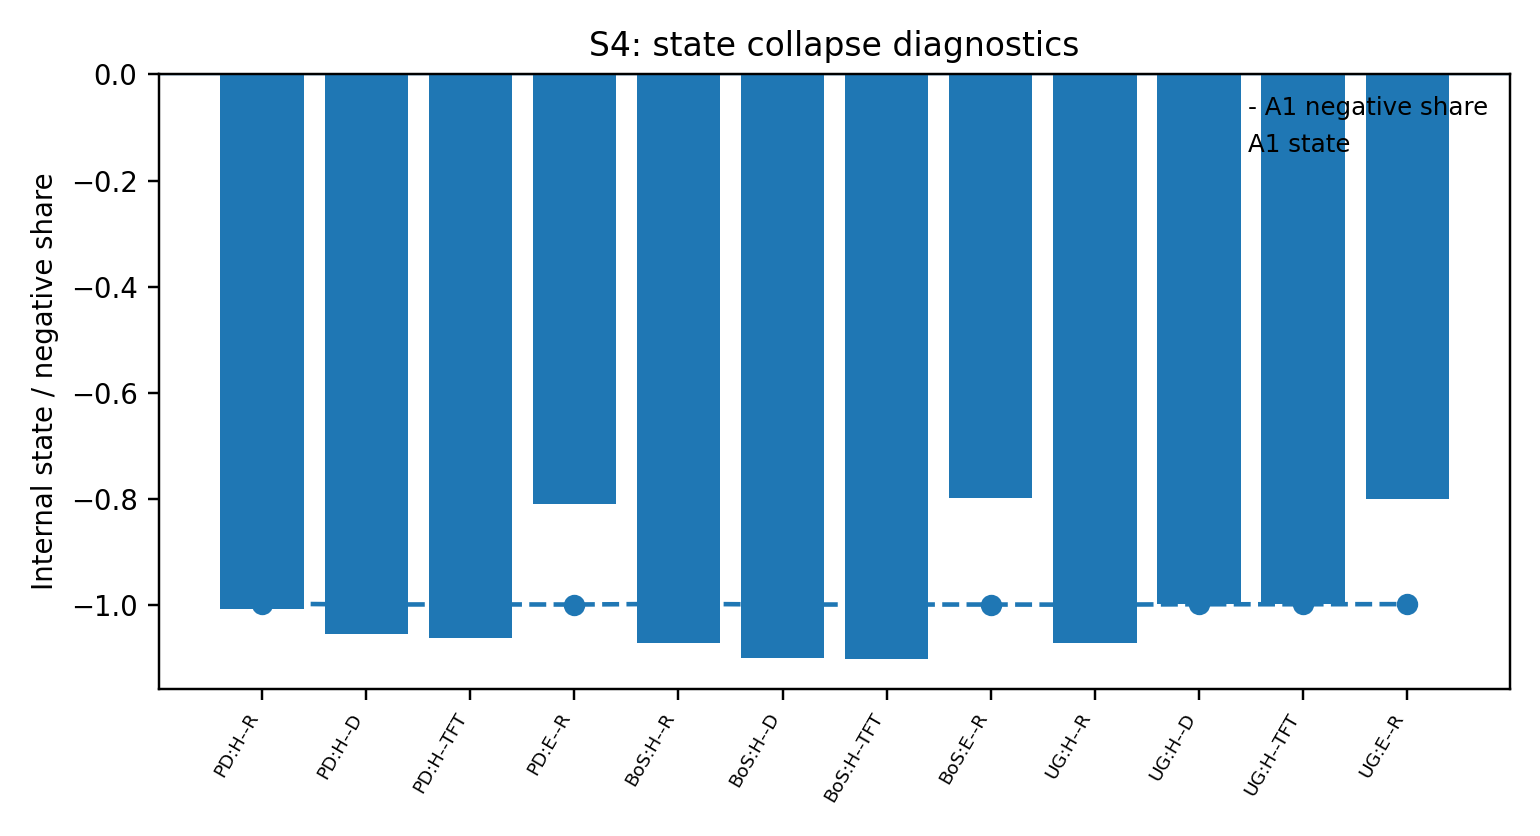
\includegraphics[width=0.80\linewidth]{figures/s4_state_collapse_diagnostics.png}
\caption{S4 state-collapse diagnostics. Bars show agent~1 mean overall state; the dashed line shows the negative-state share with sign reversed for visual comparison.}
\label{fig:s4collapse}
\end{figure}

In PD, hybrid versus fixed tit-for-tat reaches higher payoff than hybrid versus always-defect, but both remain in a highly negative internal-state regime. In PD and BoS, emotional-versus-rational often has a less negative affective-agent state than hybrid-versus-rational despite similar or higher payoff in the latter. In UG, hybrid/emotional versus rational conditions have high payoff, while fixed-strategy conditions have zero payoff and are best treated as baseline artifacts. Overall, S4 answers RQ4 by showing that collapse is not merely a payoff failure. It reflects the interaction of negative appraisal, fatigue, and the linear state aggregation. Taken together, Section~6 answers the four research questions descriptively: RQ1 is supported by a common specification and runner across three games; RQ2 shows metric-dependent differences rather than dominance; RQ3 is supported only as a fixed-partner first/last-third proxy; and RQ4 is supported by repeated evidence of payoff--state divergence and chronic negative-state regimes.

\section{Discussion}

The paper-profile runs strengthen the empirical basis of the article because they replace isolated traces with reproducible multi-seed scenarios. The key scientific point is not that one agent type wins. It is that repeated-game behavior can look different depending on whether the evaluator attends to external payoff, social game metrics, or internal state. This is precisely the gap that the game-to-values framing is meant to expose.

For RQ1, the same conceptual specification was applied to the Prisoner's Dilemma, Battle of the Sexes, and Ultimatum Game. The games differ in their external meanings--cooperation, coordination, and bargaining--but they can still be mapped into material, fairness, relationship, and safety dimensions. This supports the architectural portability of the specification, while leaving empirical validation of the adapter proxies for future work.

For RQ2, the results show metric-dependent differences rather than dominance. Hybrid--rational conditions in PD and UG can produce high pair payoff, yet the affective agent's internal state remains negative and the payoff split can be asymmetric. Rational agents often look stronger under payoff and less fragile under the current internal-state score. Emotional agents sometimes show less negative state than hybrids under similar payoff. These findings are not a failure of the article's framing; they are the diagnostic object of the paper.

For RQ3, S2 provides only a narrow adaptation proxy. The first-vs-last-third comparison shows measurable changes, especially in PD, but it does not replace a partner-switching experiment. Rational adaptation is mostly payoff-oriented, while affective adaptation is mixed. For RQ4, the central finding is that the current implementation exposes calibration failures instead of hiding them: fixed high targets, fatigue accumulation, and the linear state aggregation can generate chronic negative-state regimes even when payoff is non-trivial.

The most important boundary is implementation status. Mood, fatigue, well-being, and the learned control flow affect the reported runs. The adapter and appraisal layer are used here to interpret and diagnose outcomes from logs. Future components such as a white-box bounded-rational agent and explicit belief update should be evaluated in later ablation studies, not read back into the present evidence.

\section{Reproducibility and Artifacts}

The artifact bundle contains the LaTeX source, bibliography, generated tables and figures, the latest corrected agent code, experiment runner, configuration files, analyzed paper-run tables, selected figures, the experiment report, run inventory, adaptation diagnostics, collapse diagnostics, and interpretation guardrails. The code snapshot includes learned agent modules, rational and fixed-strategy baselines, runner/configuration utilities, metrics, plotting code, and the diagnostic adapter.

The paper-profile runs used here were executed as S1--S4 with 20 episodes and 200 rounds. A representative command is:
\begin{verbatim}
python experiment_runner.py --scenario S1 \
    --profile paper --games all --yes
\end{verbatim}
The artifact also includes a reproduction-oriented runner and selected CSV sources; figures and tables can be regenerated from saved run outputs without changing the reported values. All reported tables should be interpreted as descriptive means and diagnostics. We do not report significance tests because the experiments are still primarily calibration-oriented and because several fixed-strategy conditions are meaningful only as stress tests.

\section{Threats to Validity and Scope}

The main threats are methodological rather than rhetorical: the runs are descriptive, the learned modules are not claimed to be converged, the internal-state score is a diagnostic construct, and several formal components are explanatory rather than behavior-driving in the current implementation.

First, although 20 episodes per condition are a substantial improvement over the previous diagnostic traces, the results remain calibration-oriented. We therefore avoid p-values and superiority language. Second, even 200-round episodes are short relative to standard deep-RL training regimes; the DQN-like modules should be read as trainable prototype policies. Third, the rational baseline does not experience the same affective load as the hybrid agent. Symmetric baselines with comparable state costs and ablations without mood, fatigue, refocus, or value diagnostics are needed.

Fourth, the game-to-values adapter uses engineering proxies for fairness, relationship quality, and safety. These proxies are interpretable but not validated against human judgments. Fifth, fixed-strategy conditions are cleanest in PD; in UG, some fixed-strategy cells produce zero payoff and are treated as technical stress tests. Sixth, the overall state $S_i=w_i+m_i-f_i$ is a transparent diagnostic aggregation, not a psychometric well-being scale. Finally, the three games are diagnostic testbeds rather than a comprehensive model of organizational behavior, and no human-subject data or observer judgments are used. Claims about human-like behavior therefore remain outside the current evidence.

\section{Conclusion}

We presented an implementation-aware specification of emotionally bounded-rational agents for repeated games and evaluated it with new paper-profile diagnostic runs. The architecture separates external outcomes from internal value interpretation, connects value changes to appraisal and regulation, and exposes how mood, fatigue, and well-being can influence action selection. The experiments do not show robust dominance of hybrid agents over simpler baselines: fixed TFT is the PD sanity-check optimum, hybrid--rational conditions can be high-payoff but asymmetric and negative in internal state, and all S3 profile cells remain mostly negative. Their value lies elsewhere: they reveal payoff--state divergence, adaptation limits, internal-state collapse, and the importance of distinguishing behavior-driving mechanisms from diagnostic layers. This makes the article a calibration study and a reproducible foundation for ablations, longer runs, a future white-box bounded-rational baseline with explicit belief update, and human-data validation.

\section*{Acknowledgments}
We thank the reviewers for comments that helped reframe the work as a diagnostic calibration study and improve the formal model. Generative AI tools were used for language polishing, structural revision support, and artifact organization; modeling decisions, experiment interpretation, and final scientific claims were reviewed and approved by the authors.

\section*{Disclosure of Interests}
The authors declare no competing interests.

\section*{Supplementary Material Statement}
The artifact bundle includes the S3 per-cell profile table, reviewer-facing reproducibility checklist, full source CSV files, selected figures, run logs, code snapshot, and experiment report. These materials are not used to introduce stronger claims than those stated in the main paper.

\bibliographystyle{splncs04}
\bibliography{eumas2026_references_v8}

\end{document}
